%%%%%%%%%%%%%%%%%%%%%%%%%%%%%%%%%%%%%%%%%%%%%%%%%%%%%%%%%%%%
%%% ELIFE ARTICLE TEMPLATE
%%%%%%%%%%%%%%%%%%%%%%%%%%%%%%%%%%%%%%%%%%%%%%%%%%%%%%%%%%%%
%%% PREAMBLE 
\documentclass[9pt]{NEU502b-fmri}
% Use the onehalfspacing option for 1.5 line spacing
% Use the doublespacing option for 2.0 line spacing
% Please note that these options may affect formatting.
% Additionally, the use of the \newcommand function should be limited.

\usepackage[version=4]{mhchem}
\usepackage{array,multirow}
\usepackage{hyperref}
\usepackage{graphicx}
\usepackage[parfill]{parskip}
\usepackage{siunitx}
\DeclareSIUnit\Molar{M}

%%%%%%%%%%%%%%%%%%%%%%%%%%%%%%%%%%%%%%%%%%%%%%%%%%%%%%%%%%%%
%%% ARTICLE SETUP
%%%%%%%%%%%%%%%%%%%%%%%%%%%%%%%%%%%%%%%%%%%%%%%%%%%%%%%%%%%%

\title{BOLD Signal and Task-Correlated Respiratory Events}
\author[1]{Sam Zorowitz}

%%%%%%%%%%%%%%%%%%%%%%%%%%%%%%%%%%%%%%%%%%%%%%%%%%%%%%%%%%%%
%%% ARTICLE START
%%%%%%%%%%%%%%%%%%%%%%%%%%%%%%%%%%%%%%%%%%%%%%%%%%%%%%%%%%%%

\begin{document}

\maketitle

\begin{abstract}
We investigate the effects of task-correlated respiration on the detection and estimation of fMRI BOLD signal changes. Through a series of experiments involving visual stimulation, breath-holding, and hyperventilation, we find task-correlated respiratory events result in extensive detection of false-positive activations and reduced ability to resolve true BOLD signal change in visual cortex. We also find that a common method for de-noising respiratory artifact, CompCor, is only partially able to improve detection and estimation power. Recommendations for future research are discussed.
\end{abstract}

\section{Introduction}

The goal of functional magnetic resonance imaging (fMRI) is to measure variation in the blood oxygenation level dependent (BOLD) signal as a proxy for changes in neural activity. BOLD measurement is stymied by the fact that the signals of interest are frequently smaller in amplitude than noise arising from the scanner and participant (Huettel et al., 2004; Caballero-Gaudes and Reynolds, 2017). 

Subject respiration is one source of fMRI noise mediated by changes in arterial levels of carbon dioxide. Respiratory events can be categorized as hypercapnic (i.e. an increase in arterial CO\textsubscript{2}) or hypocapnic (i.e. a decrease in arterial CO\textsubscript{2}). Previous research has shown that induced hypercapnic events (e.g. breath-holding) results in substantial increases in the whole-brain BOLD signal (Kastrup et al., 1999a, 1999b), whereas induced hypocapnic events (e.g. hyperventilation) results in substantial decreases (Bright et al., 2009). Even small, naturally-occurring changes in breathing patterns cause measurable deflections of the BOLD signal (Van den Aardweg and Karemaker, 2002; Wise et al., 2004; Birn et al., 2006; Bianciardi et al., 2009a, 2009b). Despite this, previous studies have found that respiratory (and related cardiac signals) account for less than 10\% of the BOLD noise on average over the whole brain (Shmueli et al., 2007; Bianciardi et al., 2009a, 2009b). As such, most task-based fMRI studies ignore respiratory noise during analysis.

More recently, the neuroimaging community has shown renewed interest in controlling for respiratory noise in task-based fMRI analysis. One reason for this is growing awareness of task-correlated changes in breathing rate, wherein respiratory events are time-locked to an experimental event of interest (Napadow et al., 2008; Birn et al., 2009; Huijbers et al., 2014). If uncontrolled for, task-correlated respiratory events can result in spurious findings and/or mask true effects (Birn et al., 2009). A second reason is recent research suggesting a substantial proportion of head motion can be explained by transient respiratory events, e.g. inhaling/exhaling (Power et al., 2018). This has prompted calls for new research to better characterize and treat respiratory artifact for task-based fMRI data (Kundu et al., 2013; Power et al., 2018). 

Here, we highlight the effects of induced respiratory events on measured BOLD signal. Specifically we measure the effects of breath-holding (hypercapnic) and hyperventilation (hypocapnic) on BOLD signal during a visual stimulation paradigm. We find that task-correlated changes in respiration result in a considerable increase in the detection of false-positive activations and also hinder estimation of true activation. a common method for de-noising respiratory artifact, CompCor (Behzadi et al., 2007), is only partially able to improve detection and estimation power.

\section{Results}
The effects of task-correlated respiratory artifact was measured in two participants. Participants each completed five runs of functional scanning. In the first run, participants viewed flashing, rotating visual checkerboards (condition: \textbf{VZ}). Next, participants viewed the same stimuli while either holding their breath (condition: \textbf{V-BH}) or hyperventilating (condition: \textbf{V-HV}). For each run, the cortical response to the visual stimulus was estimated via regression with an idealized stimulus response function (see Methods for complete details). Two additional runs were collected to measure the change in BOLD signal to breath-holding (condition: \textbf{BH}) and hyperventilation (condition: \textbf{HV}) in isolation. 

\subsection{Checkerboard stimuli selectively activate visual cortex}
To understand the impact of respiration on BOLD signal, we must first establish a baseline. In the visual stimulation condition (\textbf{VZ}), participants viewed visual checkerboard stimuli in six blocks of 20s. We then regressed an idealized stimulus response against the BOLD timeseries measured at each voxel. Visual stimulation resulted in robust bilateral activation of the visual cortex for both participants (Figure 1). Anatomical masks were created from the significantly active voxels within each hemisphere separately for each participant. The average BOLD signal timeseries for each region of interest are also presented in Figure 1. In the first participant, the significantly active voxels of the left and right hemispheres exhibited an average BOLD signal increase  of 3.11\% (se = 0.33\%) and 3.13\% (se = 0.35\%), respectively. In the second participant, significantly active voxels of the left and right hemispheres exhibited a BOLD signal increase of 1.67\% (se = 0.27\%) and 1.70\% (se = 0.23\%), respectively. In sum, the checkerboard stimuli were successful in evoking robust BOLD signal change in the visual cortex of both participants. 

\begin{figure}
\centerline{%
\resizebox{1.0\textwidth}{!}{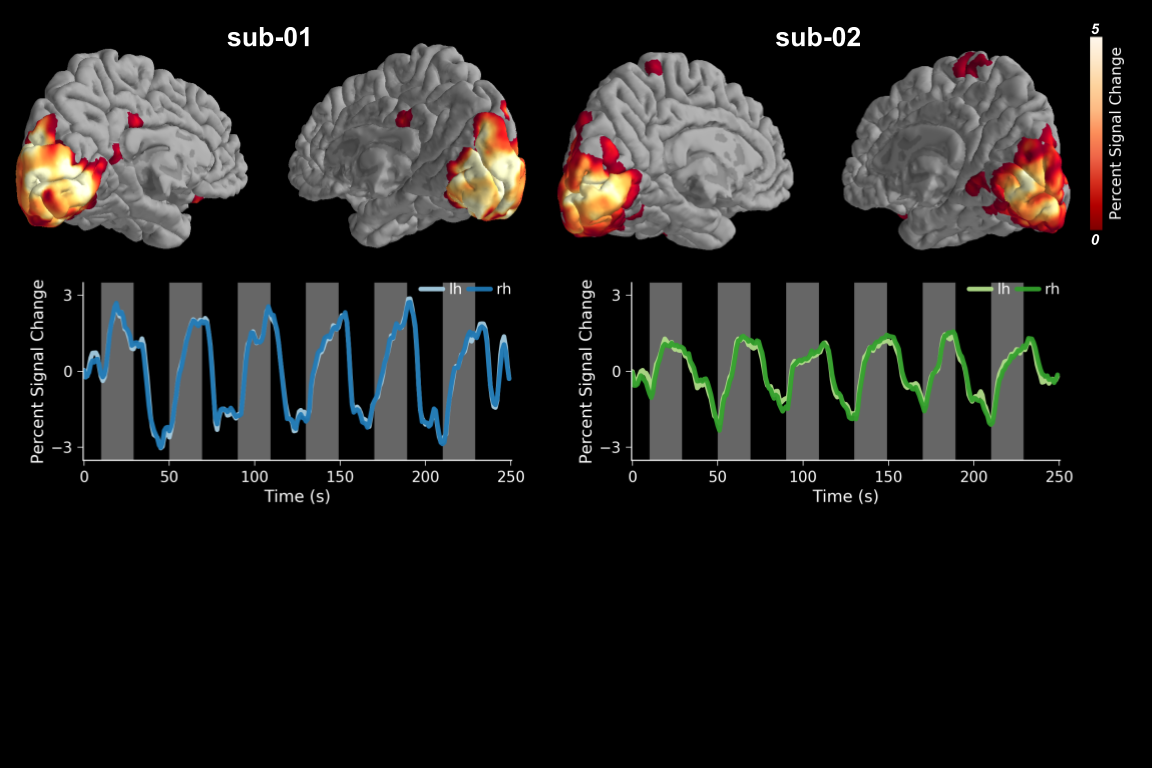
\includegraphics[trim={0 9cm 0 0},clip]{fig1.png}}%
}
\caption{\textbf{Activation maps for visual stimulation}}
\par Voxels significantly activated (i.e. increase in BOLD signal) in response to the checkerboard stimuli were selective to the visual cortex (top). BOLD signal change in visual cortex of 2-3\% was observed in both participants (bottom). 
\end{figure}

\subsection{Task-correlated respiratory events impede accurate BOLD signal measurement}
Next, we measured the cortical BOLD signal in response to to respiratory events in isolation. In the breath-holding (\textbf{BH}) and hyperventilation (\textbf{HV}) conditions, participants were instructed to hold their breaths and hyperventilate for six blocks of 20s. The averaged BOLD signal change, aligned to the onset of breath-holding/hyperventilation, are presented in Figure 2. Consistent with prior studies of hypercapnic events, breath-holding resulted in an initial reduction in BOLD signal followed by a prolonged period of BOLD signal increase, peaking around 25-30s (Kastrup et al., 1999a, 1999b; Birn et al., 2009; Bright et al., 2009). In contrast, hyperventilation resulted in an opposite pattern: an initial increase in BOLD signal followed by a prolonged period of BOLD signal decrease, peaking around 30s. This is also consistent with past research (Bright et al., 2009). These patterns of BOLD signal change were consistent across participants. 

\begin{figure}
\centerline{%
\resizebox{1.0\textwidth}{!}{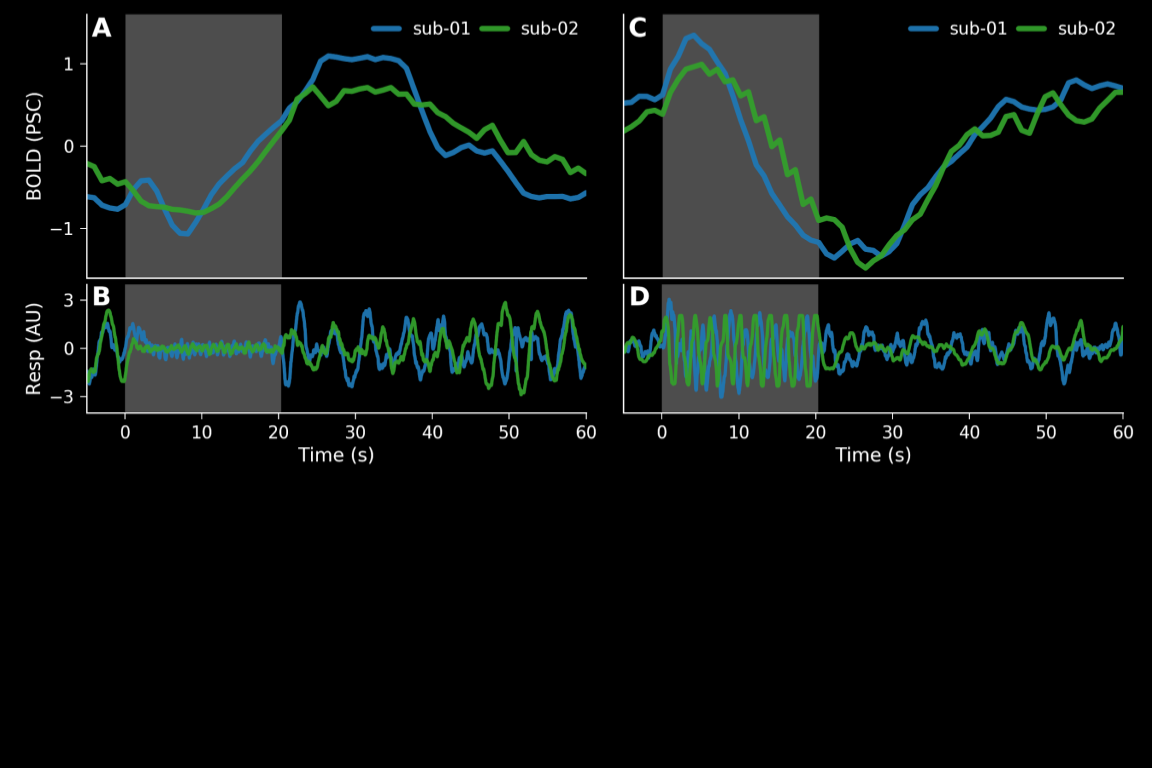
\includegraphics[trim={0 10.2cm 0 0},clip]{fig2.png}}%
}
\caption{\textbf{Effects of respiratory events on BOLD}}
\par The time-locked responses of BOLD signal to breath-holding (A) and hyperventilation (C) show consistent, opposite patterns. The corresponding physiological respiratory traces for breath-holding (B) and hyperventilation (D) are also shown. Periods of breath-holding and hyperventilation are signified by the shaded regions.

\end{figure}

Next, we investigated the effects of task-correlated respiratory events on fMRI detection power.  In the visual breath-holding (\textbf{V-BH}) and visual hyperventilation (\textbf{V-HV}) conditions, participants were again instructed to hold their breaths and hyperventilate for six blocks of 20s while viewing the same checkerboard stimuli as during visual stimulation (\textbf{VZ}). We again estimated the cortical response to the visual stimulus via regression with an idealized stimulus response function against the BOLD timeseries at each voxel. We did not include any additional regressors controlling for the respiratory events. As compared to the visual-only condition (\textbf{VZ}), significant activation was detected across the entire cortex of both participants in both conditions (Figure 3). Specifically, widespread activation (i.e. increase in BOLD signal) was detected across the cortex in the \textbf{V-BH} condition, whereas widespread deactivation (i.e. decrease in BOLD signal) was detected across the cortex n the \textbf{V-HV} condition. Insofar that the checkerboard stimuli robustly excite neurons only in visual cortex (experiment 1), these extensive significant activations are false-positives and constitute a substantial decrease in the statistical power to detect neural-in-origin changes in BOLD signal. 

Interestingly, the effects of task-correlated respiratory events are heterogeneous across both participants and cortical anatomy. For example, diffuse false-positive activation was detected across the frontal lobe of participant 1 during breath-holding, whereas comparably more sparse  false-positive activation was detected for participant 2. Similarly, false-positive deactivation was ubiquitous across the temporal and parietal lobes of participant 2 during hyperventilation, whereas false-positive deactivation was primarily located in the frontal lobe for participant 1. This suggests individual differences in the vasculature between participants, consistent with previous findings (Bright et al., 2009). 

\begin{figure}
\centerline{%
\resizebox{1.0\textwidth}{!}{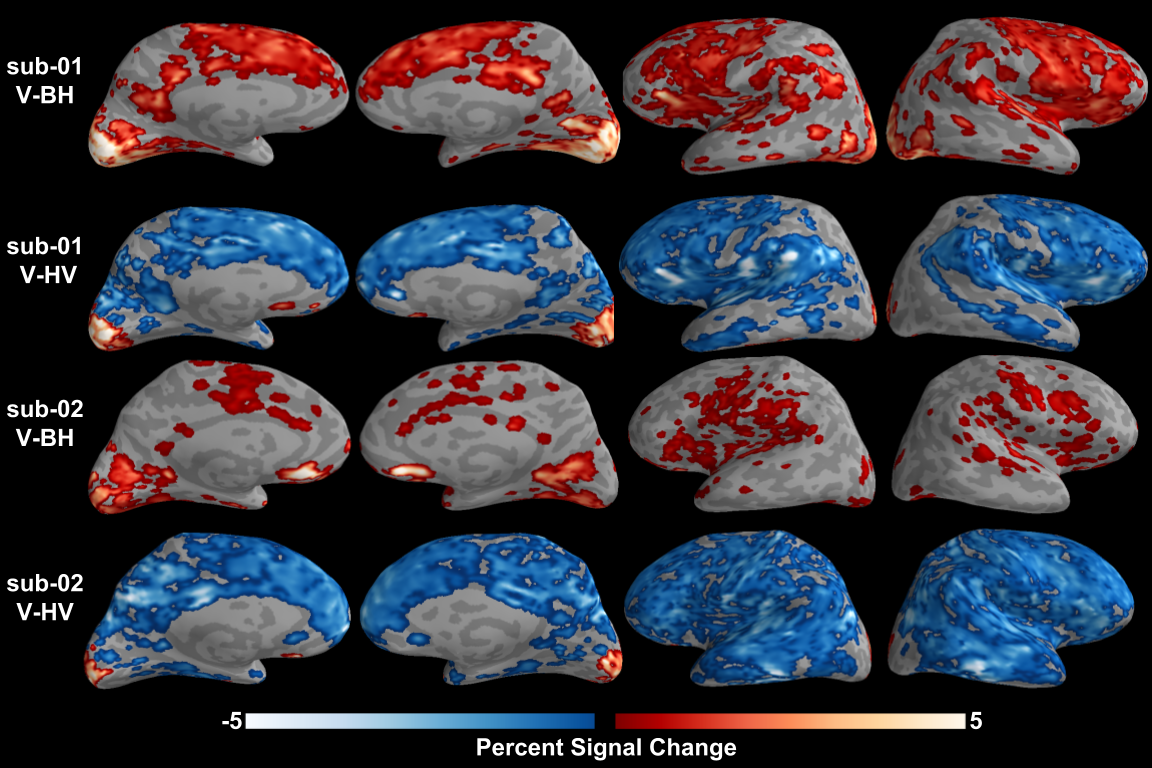
\includegraphics{fig3.png}}%
}
\caption{\textbf{Activation maps for visual breath-holding and visual hyperventilation}}
\par Widespread false-positive activations (red) and deactivations (blue) were detected in response to visual stimulation while breath-holding (V-BH) or hyperventilation (V-HV), respectively. Participants exhibit notable anatomical heterogeneity in (de)activation profiles.

\end{figure}

Next, we investigate the effects of task-correlated respiratory events on BOLD signal change estimation. Using the functionally-defined masks of visual cortex described above, we compared the estimated percent signal change in response to the checkerboard stimulus between conditions (collapsing across hemispheres within participants). The results of all pairwise contrasts are reported in Table 1.  In the first participant, a significant reduction in estimated BOLD change was observed in V-HV  as compared to VZ (F = 38.19, p < 0.001), but not in V-BH (F = 0.04, p = 0.848). In the second participant, a significant reduction in estimated BOLD was observed in both V-BH (F = 24.45, p < 0.001)  and V-HV (F = 20.94, p < 0.001) as compared to VZ. Thus, task-correlated respiratory artifact had the overall effect of impeding estimation of BOLD signal change in visual cortex during visual stimulation. 

In summary, we found that task-correlated respiratory artifact is profoundly detrimental for statistical power in task-based fMRI analysis. Breath-holding and hyperventilation during visual stimulation both resulted in widespread detection of false-positive (de)activations, as well as impeded the ability to measure true BOLD signal change. 

\begin{table}
\begin{center}
\begin{tabular}{c l l l r r}
\toprule
{Subject} & Analysis & L PSC & R PSC & F-val & p-val \\
\midrule
\multirow{5}{*}{01} & VZ          & 3.11 (0.33) & 3.13 (0.35) &       & \\
                    & V-BH           & 3.13 (0.38) & 2.98 (0.36) & 0.04  & 0.848\\
                    & V-BH + CompCor & 2.33 (0.20) & 2.25 (0.20) & 13.42 & <0.001\\
                    & V-HV           & 1.53 (0.17) & 1.41 (0.16) & 38.19 & <0.001\\
                    & V-HV + CompCor & 2.28 (0.18) & 2.16 (0.17) & 17.29 & <0.001\\\cline{2-6}
\multirow{5}{*}{02} & VZ          & 1.67 (0.27) & 1.70 (0.23) &       & \\
                    & V-BH           & 0.54 (0.23) & 0.41 (0.24) & 24.45 & <0.001\\
                    & V-BH + CompCor & 0.30 (0.14) & 0.18 (0.14) & 73.14 & <0.001\\
                    & V-HV           & 0.44 (0.14) & 1.05 (0.14) & 20.94 & <0.001\\
                    & V-HV + CompCor & 0.97 (0.13) & 1.59 (0.13) & 5.80 & 0.016 \\
\bottomrule
\end{tabular}
\end{center}
\caption{\textbf{Percent Signal Change in Visual Cortex}}
\par Summary of BOLD signal change in the visual cortex in response to visual stimulation. Percent signal change estimates with standard errors are reported across participants, hemispheres (left = L, right = R), conditions, and inclusion of respiratory nuisance regressors. The F statistics (and corresponding p-values) correspond to within-subjects pairwise contrasts estimated (averaging across hemispheres) to test for significant differences in signal change as compared to control (VZ).
\end{table}

\subsection{CompCor improves the detection and estimation of BOLD signal}

To correct for the effects of task-correlated respiratory events, we next re-estimated the regression models for the V-BH and V-HV conditions  including the CompCor regressors (Behzadi et al., 2007). Briefly, CompCor (i.e. \textit{Component Based Noise Correction}) creates nuisance regressors based on the principal components of the BOLD timeseries of the cerebrospinal fluid (CSF) and white matter (WM), where BOLD signal by definition does not reflect neural activity.  When estimating the change in BOLD signal in response to visual stimulation, the inclusion of CompCor regressors substantially reduces the number of detected false-positive (de)activations (Figure 4). Importantly including these regressors does not completely eliminate false-positive activations. Interestingly, the false-positive activations detected when including CompCor seem to be predominantly negative (i.e. decrease in BOLD signal change). The reasons for this are unclear, but may reflect differences in vasculature across the brain. 

The effects of including CompCor when estimating BOLD signal change in the visual cortex are mixed (Table 1). In both participants, the inclusion of CompCor was found to improve recovery of the true BOLD signal in visual cortex during visual stimulation and hyperventilation; in other words, the estimated BOLD signal change was larger in amplitude with CompCor, though the estimates were still significantly reduced as compared to control (participant 1: F = 17.29; p < 0.001; participant 2: F = 5.80, p = 0.016). By contrast, the inclusion of CompCor was found to decrease recovered estimates of the BOLD signal change in visual cortex during visual stimulation and breath-holding. It is not immediately clear why CompCor is more effective in correcting for hypercapnic than hypocapnic events. In summary, the inclusion of CompCor regressors provided moderate improvements in detection and estimation power for measuring BOLD signal change in the presence of task-correlated respiratory artifact.

\begin{figure}
\centerline{%
\resizebox{1.0\textwidth}{!}{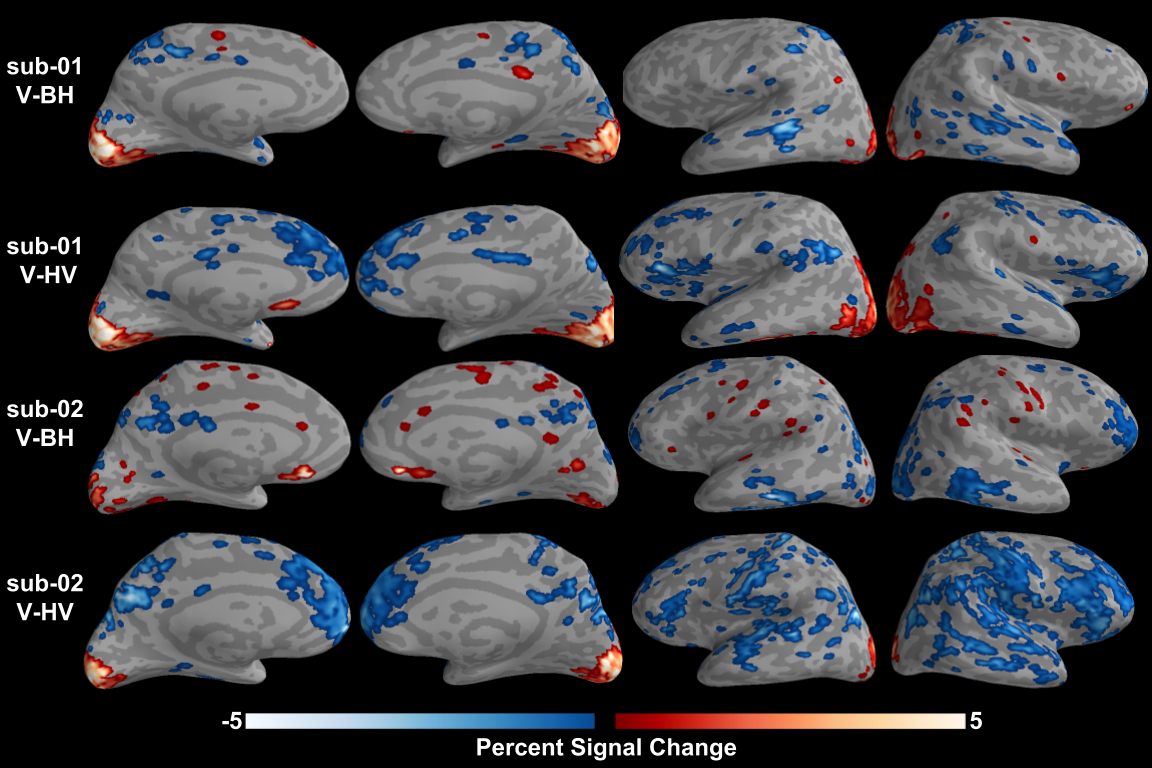
\includegraphics{fig4.png}}%
}
\caption{\textbf{Activation maps for visual breath-holding and visual hyperventilation with CompCor}}
\par The inclusion of the CompCor nuisance regressors reduces the number of false-positive activation and deactivations detected in response to visual stimulation while breath-holding (V-BH) or hyperventilating (V-HV). 

\end{figure}
Finally, for the sake of completeness, we note we attempted to create custom respiratory nuisance regressors based on the stereotyped BOLD signal responses to breath-holding and hyperventilation. We found, however, that the resulting regressors were highly collinear with the idealized checkerboard stimulus response regressor and thus unsuitable for performing regression.

\section{Discussion}
In a brief series of experiments, we investigated the effects of task-correlated respiratory events on the ability to detect and estimate fMRI BOLD signal change. We found that breath-holding and hyperventilation during visual stimulation resulted in extensive detection of false-positive (de)activations and reduced ability to estimate true BOLD signal change in visual cortex. In addition, we found that the popular CompCor nuisance regressors were only partially able to mitigate false positives and recover BOLD activation. 

The present results demonstrate the importance of controlling for task-correlated respiratory artifact. Though our experiments represent an extreme case of task-correlated respiration, they highlight the potential dangers for task-based fMRI analysis when respiratory events are ignored. One line of future research for the neuroimaging community is to develop novel methods for better removing these contaminants. Early results from using multi-echo ICA are promising (Power et al., 2018) and deserve further attention. More importantly, future studies should investigate techniques for coaching participants on proper breathing while in the fMRI scanner. After all, preventing artifact in the first place is always preferable to even the best de-noising algorithms. 

\section{Methods}

\subsection{Participants}
Two participants (both female, age 25) volunteered to participate in this experiment as part of a course on cognitive neuroscience methods. Both participants reported being right-handed and without a current or past diagnosis of a psychiatric or neurological disorder. All experimental procedures were approved by the NEU502b course instructors. 

\subsection{Task Paradigms}

\textbf{Visual Stimulation} The visual stimulation task was used to localize BOLD signal change in the visual cortex of participants. Participants viewed a rotating, flashing black-and-white checkerboard stimulus. The stimuli were presented in six 20s blocks with 20s of fixation cross in-between. The run lasted 250s and was completed once per participant.

\textbf{Breath-holding} The breath-holding task was used to measure the physiological BOLD response to a hypercapniac event. Participants were instructed to hold their breath for six blocks of 20s. Each block was followed by a recovery period of 40s. The run lasted 370s and was completed once per participant. The task was designed based on previous research (Birn et al., 2009). 

\textbf{Hyperventilate} The hyperventilation task was used to measure the physiological BOLD response to a hypocapniac event. Participants were instructed to rapidly inhale then exhale with each action lasting 2s. Participants hyperventilated for six blocks of 20s. Each block was followed by a recovery period of 40s. The run lasted 370s and was completed once per participant. The task was designed based on previous research (Bright et al., 2009). 

\textbf{Visual Breath-holding} The visual breath-holding task was designed to measure the effects of a hypercapniac event on BOLD detection during visual stimulation. Participants were instructed to hold their breath for six blocks of 20s. 10s into each each block, the checkerboard stimulus as above was presented for 20s. In other words, the breath-holding and visual stimulation blocks each lasted 20s and were staggered by 10s. Each block was followed by a recovery period of 30s. he run lasted 370s and was completed once per participant.

\textbf{Visual Hyperventilation} The visual hyperventilation task was designed to measure the effects of a hypocapnic event on BOLD detection during visual stimulation. Participants were instructed to hyperventilate as above for six blocks of 20s. 10s into each each block, the checkerboard stimulus as above was presented for 20s. In other words, the hyperventilation and visual stimulation blocks each lasted 20s and were staggered by 10s. Each block was followed by a recovery period of 30s. he run lasted 370s and was completed once per participant.

The visual stimuli were programmed in Python and Psychopy (Peirce, 2008), and were presented with a projector. Participants viewed the projection on a screen fixed at the back of the scanner bore, through a mirror fixed in front of the eyes.

\subsection{Data Acquisition}
Briefly, all images were acquired with a 64 channel head coil on a 3T Siemens Prisma. A T1-weighted MPRAGE image was acquired with TR=2530 ms,  TE 3.31 ms, flip angle=7 deg, in-plane FOV=256 x 256 mm, 176 slices, 1.0 mm isotropic voxels. For advanced anatomical registration (see below), a T2-weighted image was acquired TR=3200 ms, TE=428 ms, flip angle=120 deg, in-plane FOV=256 × 256 mm, 72 slices, 1.0 mm isotropic voxels. Whole-brain EPI acquisitions were acquired with TR=1000 ms, TE=30 ms, flip angle=55 deg, in-plane FOV=192 × 192 mm, 56 slices, 3.0 mm isotropic voxels, with a multi-band acceleration factor of 4. One run of each task was acquired with anterior-to-posterior phase encoding. Prior to the collection of the EPI images, a fieldmap was acquired for the purposes of susceptibility distortion correction (see below) with TR=1000 ms, TE=3.47 ms, flip angle=120 deg, in-plane FOV=192 × 192 mm, 56 slices, 3.0 mm isotropic voxels.

To measure cardiac and respiratory signals, a pulse oximeter and respiratory bellows were fitted to participants prior to the scanning. The pulse and respiratory signals were recorded by the scanner host computer at a sampling rate of 200 Hz and 50 Hz, respectively. The recordings were aligned with the onset of the first sync pulse using a custom script. 

\subsection{Data Preprocessing}

Results included in this manuscript come from preprocessing performed using FMRIPREP v1.0.8 (Esteban et al., 2018), a Nipype based tool (Gorgolewski et al., 2011, 2017). Each T1w (T1-weighted) volume was corrected for INU (intensity non-uniformity) using \textit{N4BiasFieldCorrection} v2.1.0  (Tustison et al., 2010) and skull-stripped using \textit{antsBrainExtraction.sh} v2.1.0 (using the OASIS template). Brain surfaces were reconstructed using \textit{recon-all} from FreeSurfer v6.0.0 (Dale et al., 1999), and the brain mask estimated previously was refined with a custom variation of the method to reconcile ANTs-derived and FreeSurfer-derived segmentations of the cortical gray-matter of Mindboggle (Klein et al., 2017). Spatial normalization to the ICBM 152 Nonlinear Asymmetrical template version 2009c (Fonov et al., 2009) was performed through nonlinear registration with the \textit{antsRegistration} tool of ANTs v2.1.0 (Avants et al., 2008), using brain-extracted versions of both T1w volume and template. Brain tissue segmentation of cerebrospinal fluid (CSF), white-matter (WM) and gray-matter (GM) was performed on the brain-extracted T1w using \textit{fast} (FSL v5.0.9) (Zhang et al., 2001).

Functional data was motion corrected using \textit{mcflirt} (FSL v5.0.9; Jenkinson et al., 2002). Slice timing was not performed in light of the task design and short repetition time. Distortion correction was performed using an implementation of the TOPUP technique (Andersson et al., 2003) using \textit{3dQwarp} (AFNI v16.2.07; Cox, 1996). This was followed by co-registration to the corresponding T1w using boundary-based registration (Greve and Fischl, 2009) with 9 degrees of freedom, using \textit{bbregister} (FreeSurfer v6.0.0). Motion correcting transformations, field distortion correcting warp, BOLD-to-T1w transformation and T1w-to-template (MNI) warp were concatenated and applied in a single step using \textit{antsApplyTransforms} (ANTs v2.1.0) using Lanczos interpolation.

Physiological noise regressors were extracted applying CompCor (Behzadi et al., 2007). Principal components were estimated for the two CompCor variants: temporal (tCompCor) and anatomical (aCompCor). A mask to exclude signal with cortical origin was obtained by eroding the brain mask, ensuring it only contained subcortical structures. Six tCompCor components were then calculated including only the top 5\% variable voxels within that subcortical mask. For aCompCor, six components were calculated within the intersection of the subcortical mask and the union of CSF and WM masks calculated in T1w space, after their projection to the native space of each functional run. Framewise displacement (Power et al., 2014) was calculated for each functional run using the implementation of Nipype.

Many internal operations of FMRIPREP use \textit{Nilearn} (Abraham et al., 2014), principally within the BOLD-processing workflow. For more details of the pipeline see \href{https://fmriprep.readthedocs.io/en/latest/workflows.html}{https://fmriprep.readthedocs.io/en/latest/workflows.html}.

Image quality was assessed using MRIQC v0.10.4 (Esteban et al., 2017). Both anatomical and functional scans were visually inspected for artifacts and showed no apparent defects. The QC reports, including carpet plots of the raw BOLD signal (Power, 2017), are included for  inspection.

\subsection{Data Analysis}
Prior to analysis, all functional data were downsampled from the native Freesurfer brain meshes (~140,000 vertices per hemisphere) to the \textit{fsaverage5} template brain (10242 vertices per hemisphere). This downsamplign procedure is approximately equivalent to applying spatial smoothing with a Gaussian kernel with FWHM of approximately 6 mm\textsuperscript{2}. To remove low frequency drift terms, functional data were high-passed filtered at 100s using Nilearn.

Activation maps in response to the visual checkerboard stimuli were estimated for the visual stimulation, visual breath-holding, and visual hyperventilation tasks by regressing the BOLD timeseries at each voxel against an idealized stimulus response function. Here, the stimulus response function was computed by convolving a boxcar function (corresponding to the onset/offset times of the visual checkerboard stimuli) with the canonical hemodynamic response function. 

For all regression analyses, motion regressors and scrubbers were included. The motion regressors were comprised of the timeseries of the six degrees of motion after being de-meaned, linearly detrended, and orthogonalized with principal components analysis. Motion scrubbers were used to regress our the effects of volumes with high motion artifact, here defined as framewise displacement (FD) > 0.5 mm as previously recommended (Power et al., 2014; Siegel et al., 2014). The motion scrubbers consist of a column of zeros except for a 1 in the row corresponding to the motion-contaminated volume. Across all runs, only 3 volumes exhibited FD > 0.5 mm. In the final regression analyses controlling for respiration artifact, the anatomical CompCor regressors estimated by FMRIPREP were used.

To correct for temporal autocorrelation, the data and design matrices were prewhitened using a Tukey taper approach (Woolrich et al., 2001). Multiple comparisons corrections across voxels were implemented via permutation testing with 5000 null permutations and family-wise error correction at alpha = 0.05 (Winkler et al., 2014). The resulting activation maps were projected back onto the native freesurfer brains for visualization. 

\nocite{*} % This command displays all refs in the bib file. PLEASE DELETE IT BEFORE YOU SUBMIT YOUR MANUSCRIPT!
\bibliography{NEU502b-fmri}

\end{document}